\subsubsection{概要}

きなこチームでも, むぎまるチーム同様, 
自己位置推定にemcl2\_ros2, ナビゲーションにnavigation2を採用したが, 
チームの目標である自己位置推定の信頼性向上のため, 
emcl2\_ros2に手を入れた. 
具体的には, 3D LiDARの3次元点群を高さ別に分け, 
それぞれの高さで2次元の地図を作り, 
走行中に利用する2次元地図を切り替えるというものである. 
これにより, たとえば人が多いところでは地上から離れた
高さの地図を使ったり, 場所ごとに
より特徴に富んだ高さの地図を使い分けたりすることができる. 
また, 地図と同じ高さのスキャンデータを使用することで, 
マップとスキャンデータの特徴の対応関係をより正確にさせている. 
3次元の自己位置推定を用いないのは, 
計算量の削減を指向したからである. 
%@@@↑あってます?

%開発の背景には, 人や車などの動的障害物による自己位置推定の破綻という課題があった. 
%当初この問題に対し, 動的障害物の影響を受けにくい2m以上の高さの点群データのみを使用する手法を採用していた. 
%自己位置推定手法はむぎまるチームと同じように, 3次元マップとセンサから得られる点群データは, 高さ方向(z軸)の情報を圧縮し2次元平面(xy平面)に投影し, 2次元マップと2次元のスキャンデータによる自己位置推定を実現していた. 
%しかし, 環境の特徴は場所によって異なる高さに存在する. 
%そのため, この手法では重要な特徴が失われ, 自己位置推定が不安定になる問題が発生していた. 
%この課題を解決するため, ロボットの現在位置に応じて自己位置推定に使用するマップとスキャンデータの高さ範囲を動的に変更するシステムを新たに開発した. 


\subsubsection{システム構成}
システムの開発のために以下の2つのパッケージを作成した. 

\begin{itemize}
  \item map\_manager: 複数の2次元マップと高さ範囲のパラメータを管理
    \begin{itemize}
      \item ロボットが指定した領域に進入すると, その領域に最適化された2次元マップと高さパラメータを提供
    \end{itemize}
  \item pointcloud\_to\_dual\_scan: 3D LiDARのスキャンデータから2種類の2次元スキャンデータを生成
        \begin{itemize}
          \item 障害物回避用のスキャンデータ
          \item 自己位置推定用のスキャンデータ(map\_managerの指定する高さ範囲に基づく)
        \end{itemize}
\end{itemize}
%!!!ここは絶対に空行をあけないこと!
map\_managerは, 事前に作成した複数の2次元占有格子地図を保持している. 
これらの地図は, 3D LiDARとIMUを統合したSLAM技術であるGLIM\cite{glim}を用いて作成した3次元マップから, 必要な高さ領域を抽出して変換したものである. 

\subsubsection{システム統合}
図\ref{fig:kinako_system}に示すように, 3D LiDARから取得したスキャンデータはpointcloud\_to\_dual\_scanで処理され, 2種類の2次元スキャンデータに変換される. 
map\_managerは, ロボットの位置に応じて最適な2次元マップと高さパラメータを提供し, 自己位置推定を安定させる. 
navigation2により生成された速度指令値はraspimouseを介してモータードライバに伝達され, ロボットの制御を実現している. 

\begin{figure}[h]
  \begin{center}
    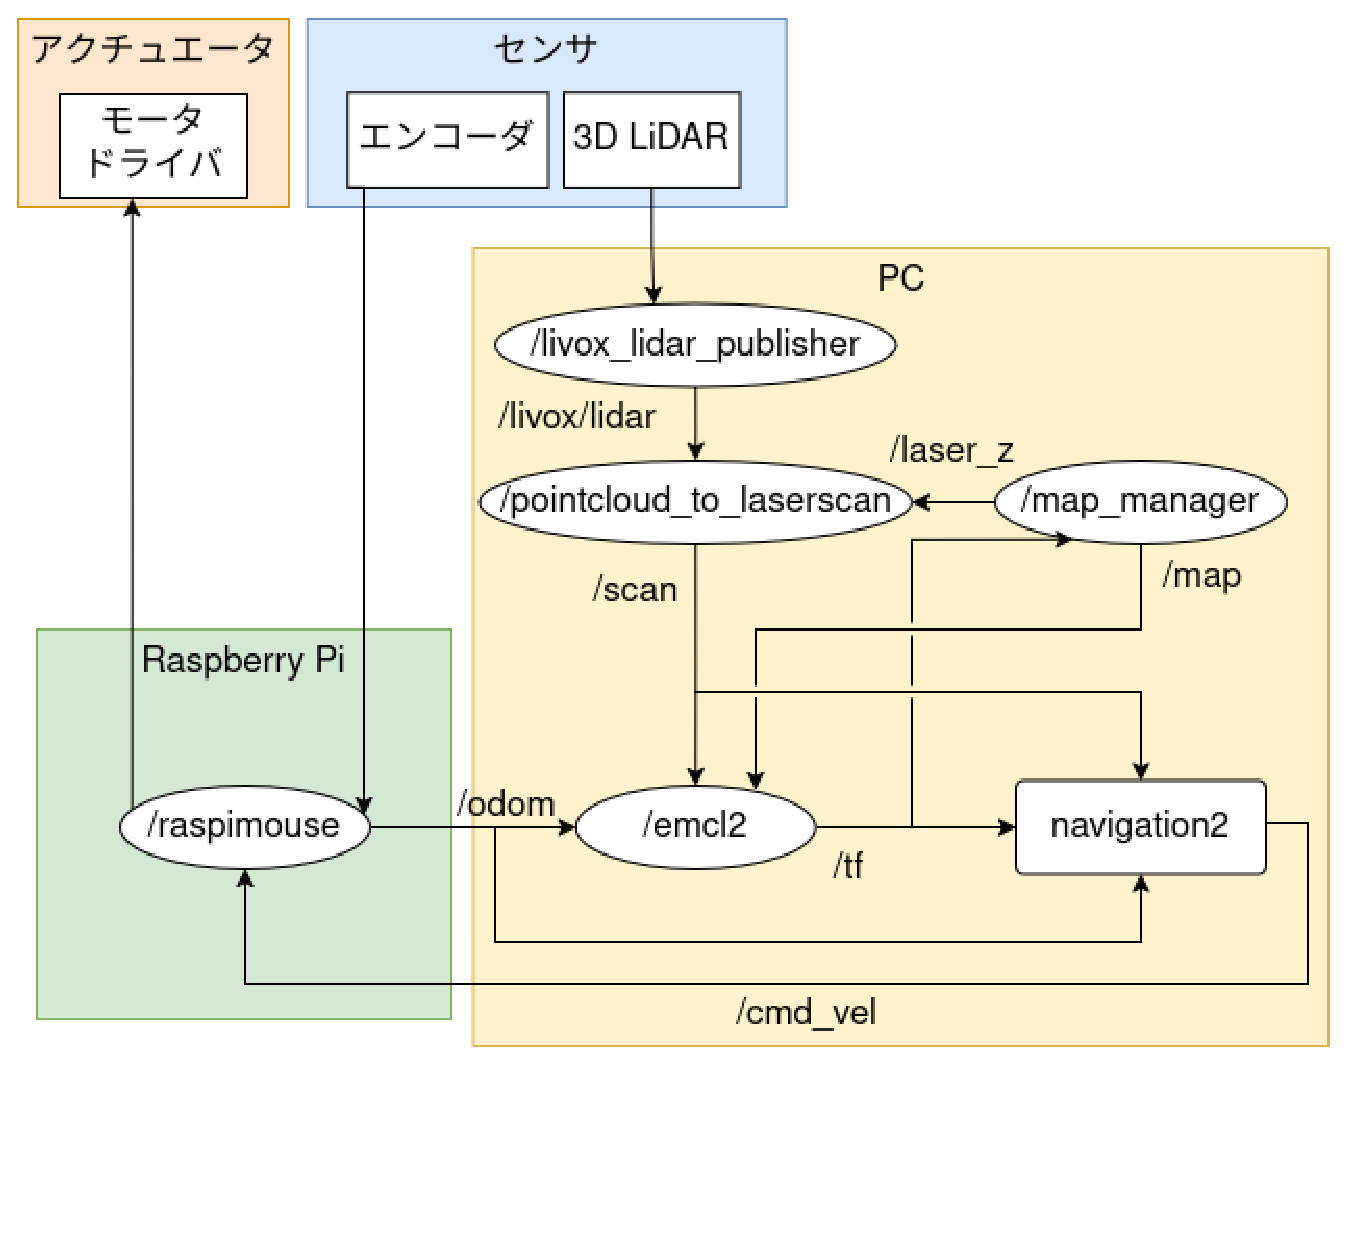
\includegraphics[width=1.0\linewidth]{figs/kinako_system_2024.eps}
    \caption{きなこチームのシステム構成}
    \label{fig:kinako_system}
  \end{center}
\end{figure}
